\section{Results: $\mnu$ shift under a lens swap}
\label{sec:results-mnu}

We now report the $\mnu$-posterior shifts induced by swapping the SPT lens (SPT2018 $\rightarrow$ SPT D1) under a fixed completion (\cref{sec:mnu-inference}). We emphasize the intended interpretation: these shifts are \emph{packaged} outputs and should be read alongside the lens-swap audits in \cref{sec:results-audits}, which localize where the two lenses disagree and test whether staging controls resolve the mismatch.

\begin{table}[t]
  \centering
  \caption{Summary of $\mnu$ shifts reproduced in this note. Values are in eV; ``Shift'' denotes (SPT2018 minus SPT D1) for the corresponding setup.}
  \label{tab:mnu-shift}
  \resizebox{\linewidth}{!}{\begin{tabular}{p{0.33\linewidth} l r r r r}
\toprule
Setup & Lens & median [eV] & 95\% upper [eV] & mode [eV] & boundary frac \\
\midrule
SPT-only + DESI DR2 BAO & SPT2018 & 0.071 & 0.194 & 0.050 & 0.00223 \\
SPT-only + DESI DR2 BAO & SPT D1 & 0.042 & 0.085 & 0.070 & 0 \\
SPT-only + DESI DR2 BAO & Shift (2018 - D1) & 0.029 & 0.109 & --- & --- \\
Planck-subset baseline + PR4 lensing + SPT + DESI DR2 BAO & SPT2018 baseline & 0.068 & 0.080 & 0.075 & 0 \\
Planck-subset baseline + PR4 lensing + SPT + DESI DR2 BAO & SPT D1 baseline & 0.054 & 0.068 & 0.054 & 0 \\
Planck-subset baseline + PR4 lensing + SPT + DESI DR2 BAO & Shift (2018 - D1) & 0.013 & 0.012 & --- & --- \\
\bottomrule
\end{tabular}
}
\end{table}

\subsection{SPT-only + DESI DR2 BAO: a large tightening under D1}
We first consider an intentionally simplified regime: the SPT TT/TE/EE likelihood alone (SPT2018 or D1) combined with DESI DR2 BAO. This setting is useful because it isolates the effect of swapping the SPT lens while holding fixed the late-time distance information. As summarized in Table~\ref{tab:mnu-shift}, the D1 lens yields a substantially tighter $\mnu$ upper bound than the 2018 lens in this regime.

Figure~\ref{fig:mnu-overlay-spt-desi} overlays the $\mnu$ posteriors for this SPT-only+DESI comparison. The qualitative effect is robust: under the same BAO likelihood and completion class, swapping SPT2018$\rightarrow$D1 tightens $\mnu$.

\begin{figure}[t]
  \centering
  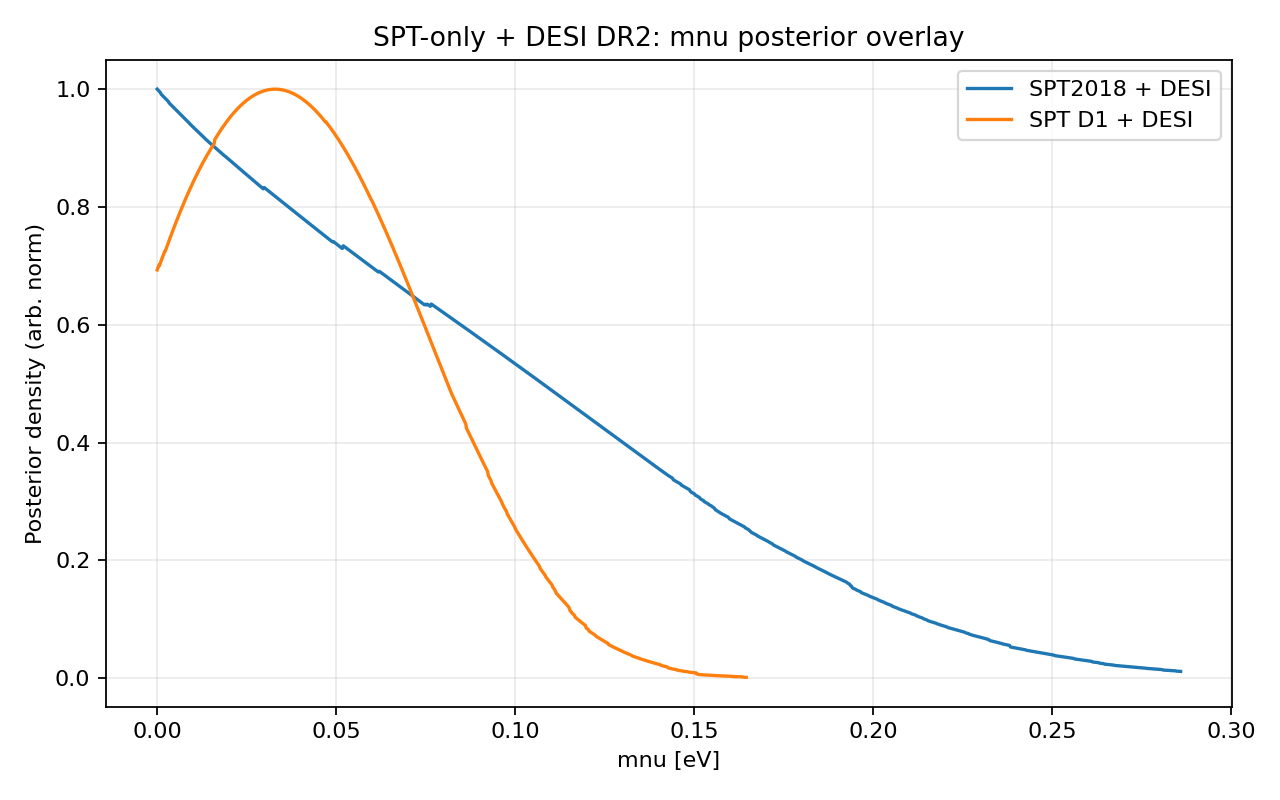
\includegraphics[width=0.85\linewidth]{figures/fig_mnu_overlay_spt_desi.png}
  \caption{$\mnu$ posterior overlay for SPT-only + DESI DR2 BAO. The D1 lens yields a tighter $\mnu$ constraint than the SPT2018 lens under the same BAO likelihood and completion. Numerical summaries are given in Table~\ref{tab:mnu-shift}.}
  \label{fig:mnu-overlay-spt-desi}
\end{figure}

\subsection{Planck-subset baseline + PR4 lensing + DESI: headline replication with a smaller shift}
We next run a baseline designed to mirror the Planck-subset+PR4-lensing structure described in \cite{arxiv2601_16277} (\cref{sec:planck-subset}), and we again combine with DESI DR2 BAO. In this setting the \emph{direction} of the lens-swap effect matches the headline behavior emphasized in \cite{arxiv2601_16277}: swapping SPT2018$\rightarrow$D1 tightens the $\mnu$ upper bound. However, the magnitude of the tightening in our reproduction is smaller than the difference between the corresponding values quoted in \cite{arxiv2601_16277} (Table~\ref{tab:mnu-shift}).
Because this baseline shift is at the $\mathcal{O}(10^{-2},\mathrm{eV})$ level, we treat it as a \emph{directional} replication: its magnitude is comparable to our seed-based stability proxy for the 95% upper bound, so we avoid over-interpreting small numerical differences.

Figure~\ref{fig:mnu-plancksubset-desi} shows the $\mnu$ posterior overlay for this baseline+DESI setting together with a compact bounds summary table. In these production runs we do not observe strong posterior piling at the physical boundary $\mnu=0$ (the boundary-fraction diagnostic is near zero), but a boundary mode can arise generically under truncation when inconsistent packaged constraints are tightened; we return to this mechanism in \cref{sec:boundary-mode}.

\begin{figure}[t]
  \centering
  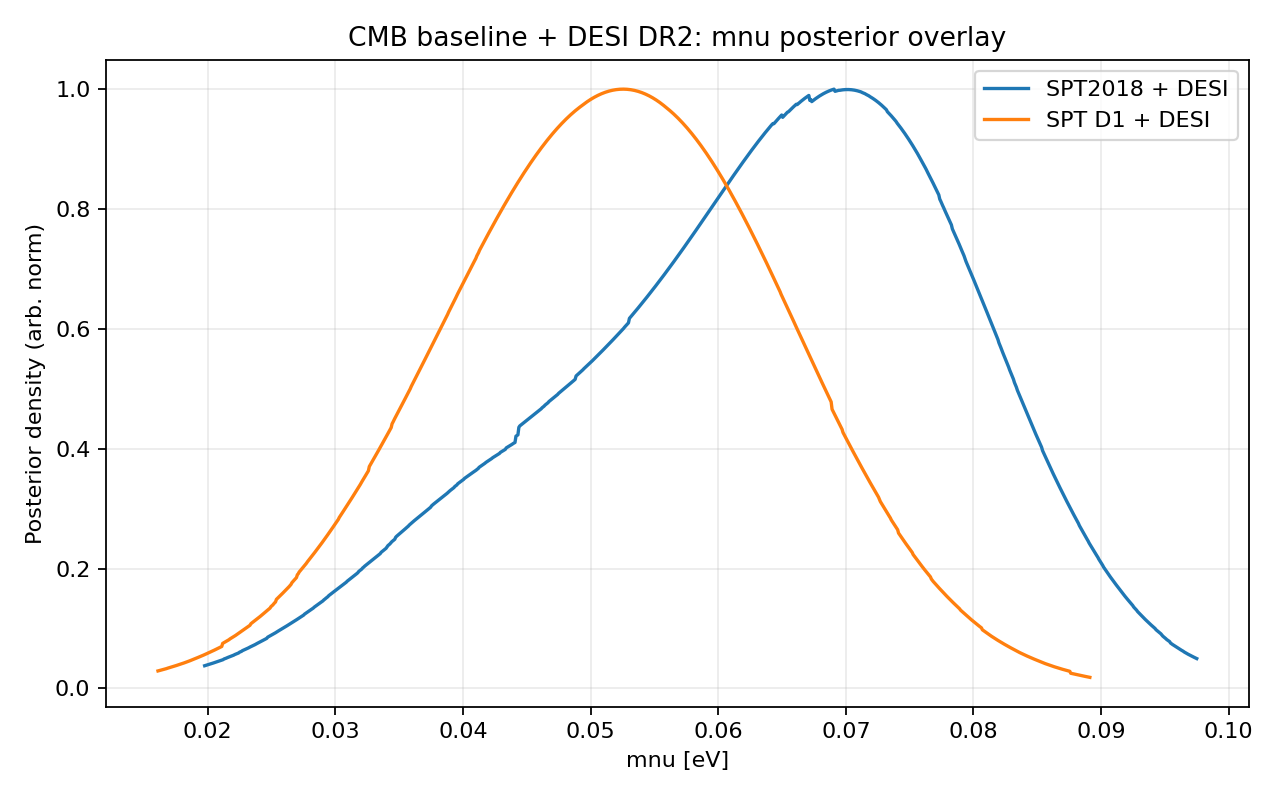
\includegraphics[width=0.85\linewidth]{figures/fig_mnu_overlay_plancksubset_desi.png}

  \vspace{6pt}
  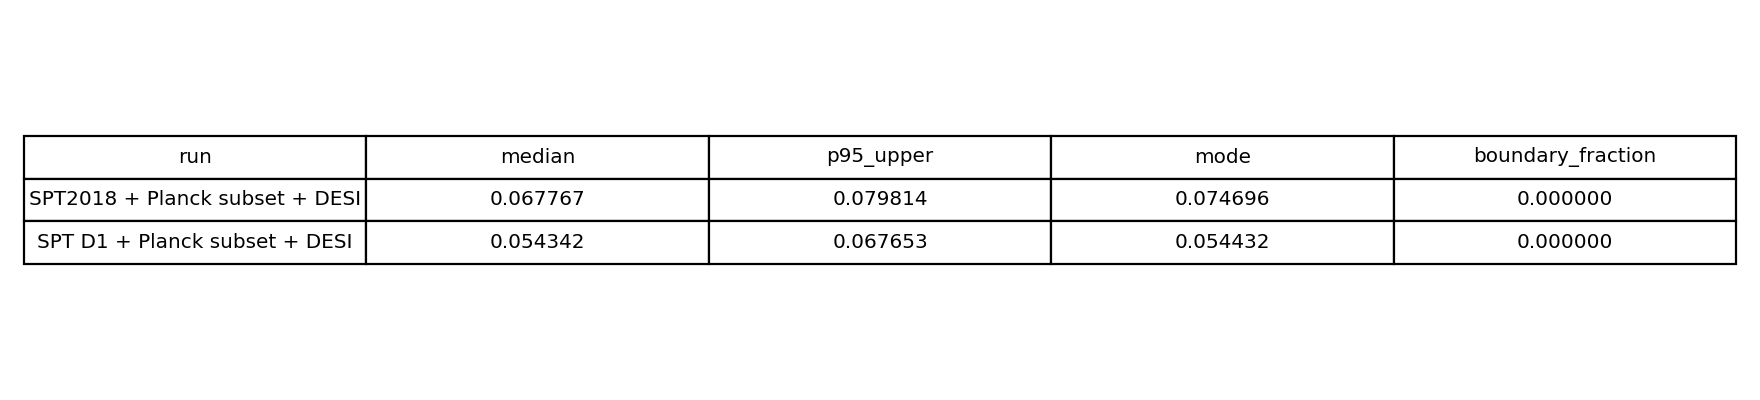
\includegraphics[width=0.85\linewidth]{figures/fig_mnu_bounds_plancksubset_desi.png}
  \caption{$\mnu$ posterior overlay (top) and bounds summary (bottom) for the Planck-subset baseline + PR4 lensing + SPT + DESI DR2 BAO setting. The D1 lens again yields a tighter $\mnu$ constraint than SPT2018, but the shift magnitude is smaller than the gap reported in \cite{arxiv2601_16277}. See Table~\ref{tab:mnu-shift} for the numerical comparison.}
  \label{fig:mnu-plancksubset-desi}
\end{figure}

\subsection{Comparison to \cite{arxiv2601_16277} and likely drivers of residual differences}
For context, \cite{arxiv2601_16277} reports 95% upper bounds of $\mnu<0.11,\mathrm{eV}$ for their SPT2018-based CMB baseline + DESI DR2 BAO, and $\mnu<0.069,\mathrm{eV}$ for the corresponding CMB-D1 baseline + DESI DR2 BAO.
Our reproduction matches the \emph{direction} highlighted in \cite{arxiv2601_16277}: under DESI DR2 BAO, swapping SPT2018$\rightarrow$D1 tightens the $\mnu$ upper bound. The \emph{magnitude} of the shift depends on details of the completion and likelihood packaging. Several plausible contributors to the remaining numerical differences (particularly in the SPT2018 baseline bound) include:
\begin{itemize}[leftmargin=*, itemsep=2pt]
  \item \textbf{Nuisance freedom and priors.} We use a deliberately minimal nuisance sampling set for computational tractability in production chains; tighter or looser bounds can result when additional nuisance parameters are varied, reparameterized, or assigned different priors.
  \item \textbf{Planck low-$\ell$ EE variant.} Our Planck subset uses the \texttt{EE\_sroll2} low-$\ell$ EE likelihood variant available in Cobaya; small baseline differences can propagate into tight derived bounds.
  \item \textbf{Likelihood and pipeline versions.} Even when dataset selections are conceptually matched, differences in released likelihood implementations, calibration conventions, and default settings can shift posteriors in the sub-0.1\,eV regime.
  \item \textbf{Baseline components.} Our baseline matches the Planck-subset and PR4 lensing structure described in \cite{arxiv2601_16277}, but exact numerical agreement can depend on whether additional baseline components (and their nuisance couplings) are included and how they are parameterized in a given code stack.
  \item \textbf{SPT lensing component.} The CMB baseline in \cite{arxiv2601_16277} includes an SPT lensing-reconstruction likelihood component; our baseline implementation does not, which can affect absolute tight bounds and may reduce the shift magnitude.
\end{itemize}
These sensitivities are precisely why we advocate pairing headline parameter bounds with explicit lens-swap audits and staging controls (\cref{sec:results-audits}): when the packaged likelihood objects disagree in localized regions of the summary statistics, parameter-level shifts should be interpreted as packaging-sensitive until the mismatch is resolved.

\subsection{Implementation caveat: sampled \texttt{mnu\_sample} and derived $\mnu$}
\label{sec:mnu-impl-caveat}
As noted in \cref{sec:mnu-inference}, our Planck-subset baseline production runs are CLASS-based and parameterize massive neutrinos via three degenerate species masses $m_{\mathrm{ncdm}}=(\mnu/3,\mnu/3,\mnu/3)$. To keep $\mnu$ explicit in chain outputs while providing CLASS the required per-species masses, we sample an internal parameter \texttt{mnu\_sample} and expose $\mnu$ as a derived parameter used for reporting and plotting. This is a bookkeeping choice for tool compatibility; it does not change the intended meaning of the reported $\mnu$ posterior.
